\documentclass[twoside]{book}

% Packages required by doxygen
\usepackage{calc}
\usepackage{doxygen}
\usepackage{graphicx}
\usepackage[utf8]{inputenc}
\usepackage{makeidx}
\usepackage{multicol}
\usepackage{multirow}
\usepackage{textcomp}
\usepackage[table]{xcolor}

% Font selection
\usepackage[T1]{fontenc}
\usepackage{mathptmx}
\usepackage[scaled=.90]{helvet}
\usepackage{courier}
\usepackage{amssymb}
\usepackage{sectsty}
\renewcommand{\familydefault}{\sfdefault}
\allsectionsfont{%
  \fontseries{bc}\selectfont%
  \color{darkgray}%
}
\renewcommand{\DoxyLabelFont}{%
  \fontseries{bc}\selectfont%
  \color{darkgray}%
}

% Page & text layout
\usepackage{geometry}
\geometry{%
  a4paper,%
  top=2.5cm,%
  bottom=2.5cm,%
  left=2.5cm,%
  right=2.5cm%
}
\tolerance=750
\hfuzz=15pt
\hbadness=750
\setlength{\emergencystretch}{15pt}
\setlength{\parindent}{0cm}
\setlength{\parskip}{0.2cm}
\makeatletter
\renewcommand{\paragraph}{%
  \@startsection{paragraph}{4}{0ex}{-1.0ex}{1.0ex}{%
    \normalfont\normalsize\bfseries\SS@parafont%
  }%
}
\renewcommand{\subparagraph}{%
  \@startsection{subparagraph}{5}{0ex}{-1.0ex}{1.0ex}{%
    \normalfont\normalsize\bfseries\SS@subparafont%
  }%
}
\makeatother

% Headers & footers
\usepackage{fancyhdr}
\pagestyle{fancyplain}
\fancyhead[LE]{\fancyplain{}{\bfseries\thepage}}
\fancyhead[CE]{\fancyplain{}{}}
\fancyhead[RE]{\fancyplain{}{\bfseries\leftmark}}
\fancyhead[LO]{\fancyplain{}{\bfseries\rightmark}}
\fancyhead[CO]{\fancyplain{}{}}
\fancyhead[RO]{\fancyplain{}{\bfseries\thepage}}
\fancyfoot[LE]{\fancyplain{}{}}
\fancyfoot[CE]{\fancyplain{}{}}
\fancyfoot[RE]{\fancyplain{}{\bfseries\scriptsize Generated on Mon Jan 15 2018 10\-:19\-:57 for Print I\-P by Doxygen }}
\fancyfoot[LO]{\fancyplain{}{\bfseries\scriptsize Generated on Mon Jan 15 2018 10\-:19\-:57 for Print I\-P by Doxygen }}
\fancyfoot[CO]{\fancyplain{}{}}
\fancyfoot[RO]{\fancyplain{}{}}
\renewcommand{\footrulewidth}{0.4pt}
\renewcommand{\chaptermark}[1]{%
  \markboth{#1}{}%
}
\renewcommand{\sectionmark}[1]{%
  \markright{\thesection\ #1}%
}

% Indices & bibliography
\usepackage{natbib}
\usepackage[titles]{tocloft}
\setcounter{tocdepth}{3}
\setcounter{secnumdepth}{5}
\makeindex

% Hyperlinks (required, but should be loaded last)
\usepackage{ifpdf}
\ifpdf
  \usepackage[pdftex,pagebackref=true]{hyperref}
\else
  \usepackage[ps2pdf,pagebackref=true]{hyperref}
\fi
\hypersetup{%
  colorlinks=true,%
  linkcolor=blue,%
  citecolor=blue,%
  unicode%
}

% Custom commands
\newcommand{\clearemptydoublepage}{%
  \newpage{\pagestyle{empty}\cleardoublepage}%
}


%===== C O N T E N T S =====

\begin{document}

% Titlepage & ToC
\hypersetup{pageanchor=false}
\pagenumbering{roman}
\begin{titlepage}
\vspace*{7cm}
\begin{center}%
{\Large Print I\-P }\\
\vspace*{1cm}
{\large Generated by Doxygen 1.8.6}\\
\vspace*{0.5cm}
{\small Mon Jan 15 2018 10:19:57}\\
\end{center}
\end{titlepage}
\clearemptydoublepage
\tableofcontents
\clearemptydoublepage
\pagenumbering{arabic}
\hypersetup{pageanchor=true}

%--- Begin generated contents ---
\chapter{Hierarchical Index}
\section{Class Hierarchy}
This inheritance list is sorted roughly, but not completely, alphabetically\-:\begin{DoxyCompactList}
\item false\-\_\-type\begin{DoxyCompactList}
\item \contentsline{section}{is\-\_\-all\-\_\-of$<$ T, U, Args...$>$}{\pageref{structis__all__of_3_01T_00_01U_00_01Args_8_8_8_4}}{}
\item \contentsline{section}{is\-\_\-one\-\_\-of$<$ T $>$}{\pageref{structis__one__of_3_01T_01_4}}{}
\end{DoxyCompactList}
\item \contentsline{section}{gen\-\_\-seq$<$ N, Is $>$}{\pageref{structgen__seq}}{}
\item \contentsline{section}{is\-\_\-all\-\_\-of$<$ T, Args $>$}{\pageref{structis__all__of}}{}
\item \contentsline{section}{is\-\_\-all\-\_\-of$<$ T, Args...$>$}{\pageref{structis__all__of}}{}
\begin{DoxyCompactList}
\item \contentsline{section}{is\-\_\-all\-\_\-of$<$ T, T, Args...$>$}{\pageref{structis__all__of_3_01T_00_01T_00_01Args_8_8_8_4}}{}
\end{DoxyCompactList}
\item \contentsline{section}{is\-\_\-one\-\_\-of$<$ T, Args $>$}{\pageref{structis__one__of}}{}
\item \contentsline{section}{is\-\_\-one\-\_\-of$<$ T, Args...$>$}{\pageref{structis__one__of}}{}
\begin{DoxyCompactList}
\item \contentsline{section}{is\-\_\-one\-\_\-of$<$ T, U, Args...$>$}{\pageref{structis__one__of_3_01T_00_01U_00_01Args_8_8_8_4}}{}
\end{DoxyCompactList}
\item \contentsline{section}{seq$<$ Is $>$}{\pageref{structseq}}{}
\item \contentsline{section}{seq$<$ Is...$>$}{\pageref{structseq}}{}
\begin{DoxyCompactList}
\item \contentsline{section}{gen\-\_\-seq$<$ 0, Is...$>$}{\pageref{structgen__seq_3_010_00_01Is_8_8_8_4}}{}
\end{DoxyCompactList}
\item true\-\_\-type\begin{DoxyCompactList}
\item \contentsline{section}{is\-\_\-all\-\_\-of$<$ T $>$}{\pageref{structis__all__of_3_01T_01_4}}{}
\item \contentsline{section}{is\-\_\-one\-\_\-of$<$ T, T, Args...$>$}{\pageref{structis__one__of_3_01T_00_01T_00_01Args_8_8_8_4}}{}
\end{DoxyCompactList}
\end{DoxyCompactList}

\chapter{Class Index}
\section{Class List}
Here are the classes, structs, unions and interfaces with brief descriptions\-:\begin{DoxyCompactList}
\item\contentsline{section}{\hyperlink{structgen__seq}{gen\-\_\-seq$<$ N, Is $>$} \\*Gen\-\_\-seq meta-\/class }{\pageref{structgen__seq}}{}
\item\contentsline{section}{\hyperlink{structgen__seq_3_010_00_01Is_8_8_8_4}{gen\-\_\-seq$<$ 0, Is...$>$} \\*Gen\-\_\-seq meta-\/class }{\pageref{structgen__seq_3_010_00_01Is_8_8_8_4}}{}
\item\contentsline{section}{\hyperlink{structis__all__of}{is\-\_\-all\-\_\-of$<$ T, Args $>$} \\*Is\-\_\-all\-\_\-of meta-\/class }{\pageref{structis__all__of}}{}
\item\contentsline{section}{\hyperlink{structis__all__of_3_01T_01_4}{is\-\_\-all\-\_\-of$<$ T $>$} \\*Is\-\_\-all\-\_\-of meta-\/class }{\pageref{structis__all__of_3_01T_01_4}}{}
\item\contentsline{section}{\hyperlink{structis__all__of_3_01T_00_01T_00_01Args_8_8_8_4}{is\-\_\-all\-\_\-of$<$ T, T, Args...$>$} \\*Is\-\_\-all\-\_\-of meta-\/class }{\pageref{structis__all__of_3_01T_00_01T_00_01Args_8_8_8_4}}{}
\item\contentsline{section}{\hyperlink{structis__all__of_3_01T_00_01U_00_01Args_8_8_8_4}{is\-\_\-all\-\_\-of$<$ T, U, Args...$>$} \\*Is\-\_\-all\-\_\-of meta-\/class }{\pageref{structis__all__of_3_01T_00_01U_00_01Args_8_8_8_4}}{}
\item\contentsline{section}{\hyperlink{structis__one__of}{is\-\_\-one\-\_\-of$<$ T, Args $>$} \\*Is\-\_\-one\-\_\-of meta-\/class }{\pageref{structis__one__of}}{}
\item\contentsline{section}{\hyperlink{structis__one__of_3_01T_01_4}{is\-\_\-one\-\_\-of$<$ T $>$} \\*Is\-\_\-one\-\_\-of meta-\/class }{\pageref{structis__one__of_3_01T_01_4}}{}
\item\contentsline{section}{\hyperlink{structis__one__of_3_01T_00_01T_00_01Args_8_8_8_4}{is\-\_\-one\-\_\-of$<$ T, T, Args...$>$} \\*Is\-\_\-one\-\_\-of meta-\/class }{\pageref{structis__one__of_3_01T_00_01T_00_01Args_8_8_8_4}}{}
\item\contentsline{section}{\hyperlink{structis__one__of_3_01T_00_01U_00_01Args_8_8_8_4}{is\-\_\-one\-\_\-of$<$ T, U, Args...$>$} \\*Is\-\_\-one\-\_\-of meta-\/class }{\pageref{structis__one__of_3_01T_00_01U_00_01Args_8_8_8_4}}{}
\item\contentsline{section}{\hyperlink{structseq}{seq$<$ Is $>$} \\*Seq meta-\/class }{\pageref{structseq}}{}
\end{DoxyCompactList}

\chapter{File Index}
\section{File List}
Here is a list of all documented files with brief descriptions\-:\begin{DoxyCompactList}
\item\contentsline{section}{\hyperlink{print__ip_8h}{print\-\_\-ip.\-h} }{\pageref{print__ip_8h}}{}
\item\contentsline{section}{{\bfseries version.\-h} }{\pageref{version_8h}}{}
\end{DoxyCompactList}

\chapter{Class Documentation}
\hypertarget{structgen__seq}{\section{gen\-\_\-seq$<$ N, Is $>$ Struct Template Reference}
\label{structgen__seq}\index{gen\-\_\-seq$<$ N, Is $>$@{gen\-\_\-seq$<$ N, Is $>$}}
}


\hyperlink{structgen__seq}{gen\-\_\-seq} meta-\/class.  




{\ttfamily \#include $<$print\-\_\-ip.\-h$>$}



\subsection{Detailed Description}
\subsubsection*{template$<$std\-::size\-\_\-t N, std\-::size\-\_\-t... Is$>$struct gen\-\_\-seq$<$ N, Is $>$}

\hyperlink{structgen__seq}{gen\-\_\-seq} meta-\/class. 

It's stops recursion meta-\/function. \begin{DoxyReturn}{Returns}
sequence of integer numbers \mbox{[}K..N\mbox{]} 
\end{DoxyReturn}


The documentation for this struct was generated from the following file\-:\begin{DoxyCompactItemize}
\item 
\hyperlink{print__ip_8h}{print\-\_\-ip.\-h}\end{DoxyCompactItemize}

\hypertarget{structgen__seq_3_010_00_01Is_8_8_8_4}{\section{gen\-\_\-seq$<$ 0, Is...$>$ Struct Template Reference}
\label{structgen__seq_3_010_00_01Is_8_8_8_4}\index{gen\-\_\-seq$<$ 0, Is...$>$@{gen\-\_\-seq$<$ 0, Is...$>$}}
}


\hyperlink{structgen__seq}{gen\-\_\-seq} meta-\/class.  




{\ttfamily \#include $<$print\-\_\-ip.\-h$>$}

Inheritance diagram for gen\-\_\-seq$<$ 0, Is...$>$\-:\begin{figure}[H]
\begin{center}
\leavevmode
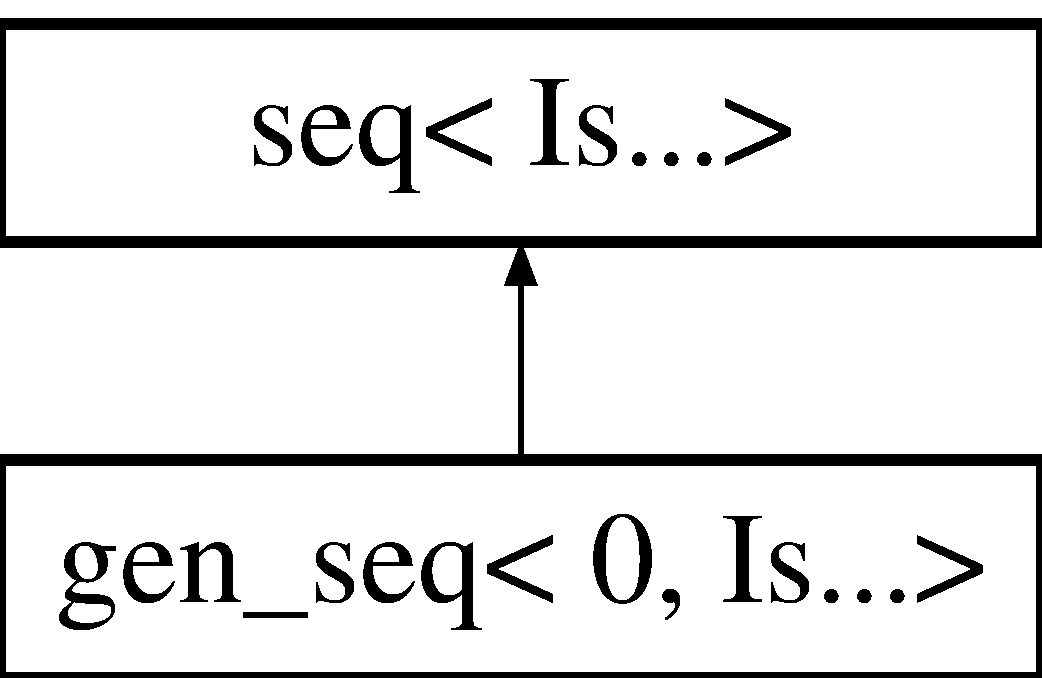
\includegraphics[height=2.000000cm]{structgen__seq_3_010_00_01Is_8_8_8_4}
\end{center}
\end{figure}


\subsection{Detailed Description}
\subsubsection*{template$<$std\-::size\-\_\-t... Is$>$struct gen\-\_\-seq$<$ 0, Is...$>$}

\hyperlink{structgen__seq}{gen\-\_\-seq} meta-\/class. 

Meta-\/function generates sequence of integer numbers. \begin{DoxyReturn}{Returns}
sequence of integer numbers \mbox{[}0..N\mbox{]} 
\end{DoxyReturn}


The documentation for this struct was generated from the following file\-:\begin{DoxyCompactItemize}
\item 
\hyperlink{print__ip_8h}{print\-\_\-ip.\-h}\end{DoxyCompactItemize}

\hypertarget{structis__all__of}{\section{is\-\_\-all\-\_\-of$<$ T, Args $>$ Struct Template Reference}
\label{structis__all__of}\index{is\-\_\-all\-\_\-of$<$ T, Args $>$@{is\-\_\-all\-\_\-of$<$ T, Args $>$}}
}


\hyperlink{structis__all__of}{is\-\_\-all\-\_\-of} meta-\/class.  




{\ttfamily \#include $<$print\-\_\-ip.\-h$>$}



\subsection{Detailed Description}
\subsubsection*{template$<$typename T, typename... Args$>$struct is\-\_\-all\-\_\-of$<$ T, Args $>$}

\hyperlink{structis__all__of}{is\-\_\-all\-\_\-of} meta-\/class. 

A basic class of \hyperlink{structis__all__of}{is\-\_\-all\-\_\-of} meta-\/function. 

The documentation for this struct was generated from the following file\-:\begin{DoxyCompactItemize}
\item 
\hyperlink{print__ip_8h}{print\-\_\-ip.\-h}\end{DoxyCompactItemize}

\hypertarget{structis__all__of_3_01T_01_4}{\section{is\-\_\-all\-\_\-of$<$ T $>$ Struct Template Reference}
\label{structis__all__of_3_01T_01_4}\index{is\-\_\-all\-\_\-of$<$ T $>$@{is\-\_\-all\-\_\-of$<$ T $>$}}
}


\hyperlink{structis__all__of}{is\-\_\-all\-\_\-of} meta-\/class.  




{\ttfamily \#include $<$print\-\_\-ip.\-h$>$}

Inheritance diagram for is\-\_\-all\-\_\-of$<$ T $>$\-:\begin{figure}[H]
\begin{center}
\leavevmode
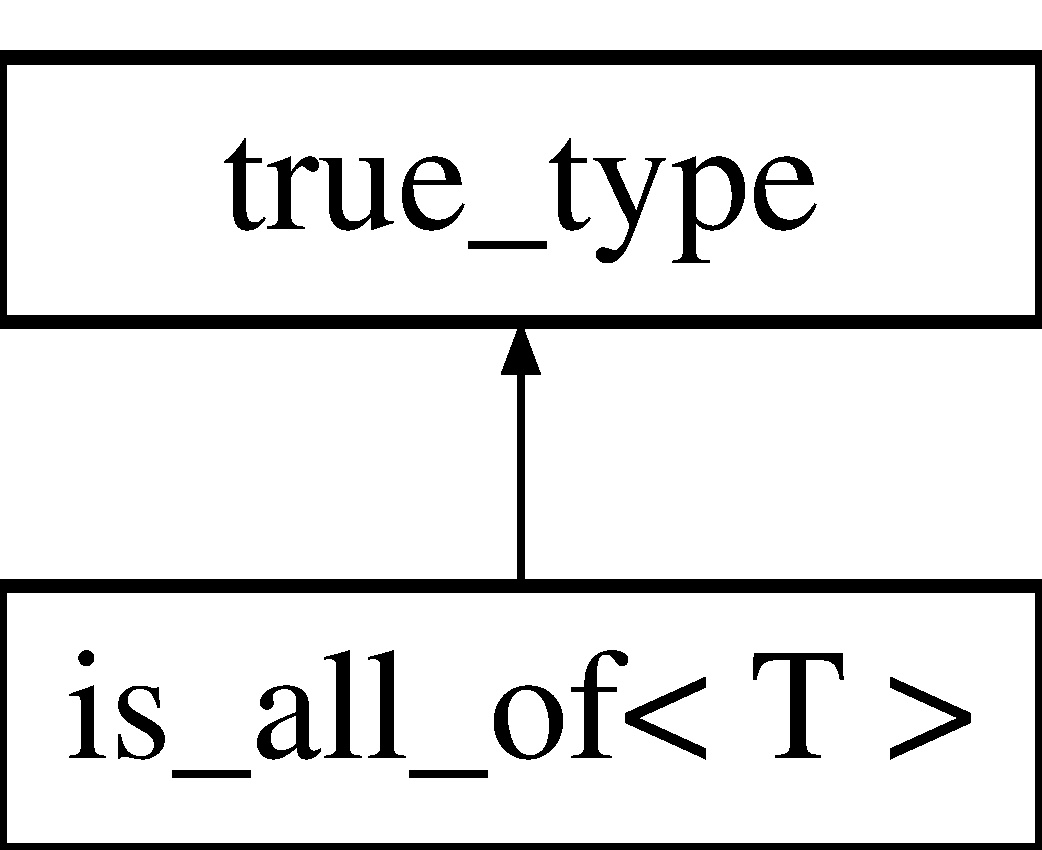
\includegraphics[height=2.000000cm]{structis__all__of_3_01T_01_4}
\end{center}
\end{figure}


\subsection{Detailed Description}
\subsubsection*{template$<$typename T$>$struct is\-\_\-all\-\_\-of$<$ T $>$}

\hyperlink{structis__all__of}{is\-\_\-all\-\_\-of} meta-\/class. 

No parameters. \begin{DoxyReturn}{Returns}
false 
\end{DoxyReturn}


The documentation for this struct was generated from the following file\-:\begin{DoxyCompactItemize}
\item 
\hyperlink{print__ip_8h}{print\-\_\-ip.\-h}\end{DoxyCompactItemize}

\hypertarget{structis__all__of_3_01T_00_01T_00_01Args_8_8_8_4}{\section{is\-\_\-all\-\_\-of$<$ T, T, Args...$>$ Struct Template Reference}
\label{structis__all__of_3_01T_00_01T_00_01Args_8_8_8_4}\index{is\-\_\-all\-\_\-of$<$ T, T, Args...$>$@{is\-\_\-all\-\_\-of$<$ T, T, Args...$>$}}
}


\hyperlink{structis__all__of}{is\-\_\-all\-\_\-of} meta-\/class.  




{\ttfamily \#include $<$print\-\_\-ip.\-h$>$}

Inheritance diagram for is\-\_\-all\-\_\-of$<$ T, T, Args...$>$\-:\begin{figure}[H]
\begin{center}
\leavevmode
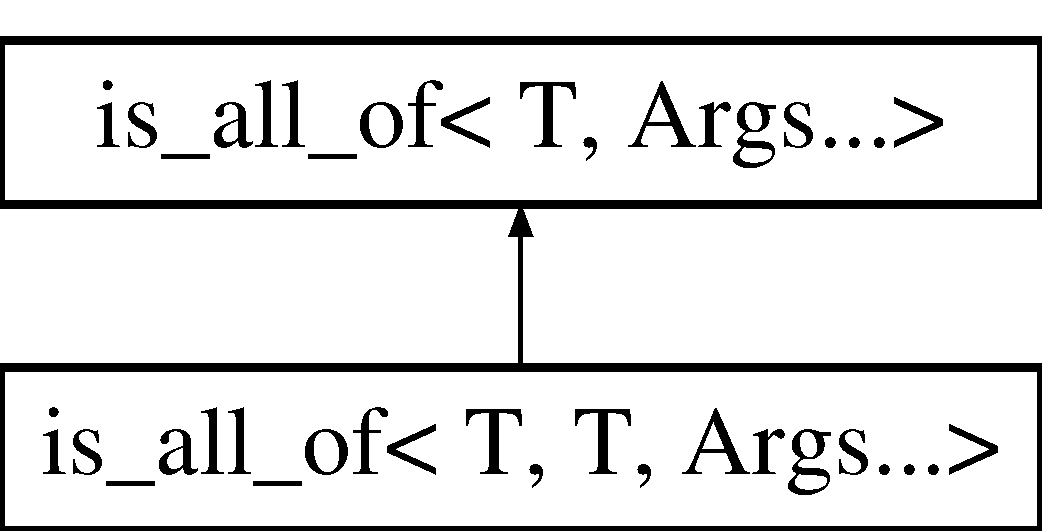
\includegraphics[height=2.000000cm]{structis__all__of_3_01T_00_01T_00_01Args_8_8_8_4}
\end{center}
\end{figure}


\subsection{Detailed Description}
\subsubsection*{template$<$typename T, typename... Args$>$struct is\-\_\-all\-\_\-of$<$ T, T, Args...$>$}

\hyperlink{structis__all__of}{is\-\_\-all\-\_\-of} meta-\/class. 

Inputs parameter and first parameter are not equal. \begin{DoxyReturn}{Returns}
next compared inputs parameter with second parameter 
\end{DoxyReturn}


The documentation for this struct was generated from the following file\-:\begin{DoxyCompactItemize}
\item 
\hyperlink{print__ip_8h}{print\-\_\-ip.\-h}\end{DoxyCompactItemize}

\hypertarget{structis__all__of_3_01T_00_01U_00_01Args_8_8_8_4}{\section{is\-\_\-all\-\_\-of$<$ T, U, Args...$>$ Struct Template Reference}
\label{structis__all__of_3_01T_00_01U_00_01Args_8_8_8_4}\index{is\-\_\-all\-\_\-of$<$ T, U, Args...$>$@{is\-\_\-all\-\_\-of$<$ T, U, Args...$>$}}
}


\hyperlink{structis__all__of}{is\-\_\-all\-\_\-of} meta-\/class.  




{\ttfamily \#include $<$print\-\_\-ip.\-h$>$}

Inheritance diagram for is\-\_\-all\-\_\-of$<$ T, U, Args...$>$\-:\begin{figure}[H]
\begin{center}
\leavevmode
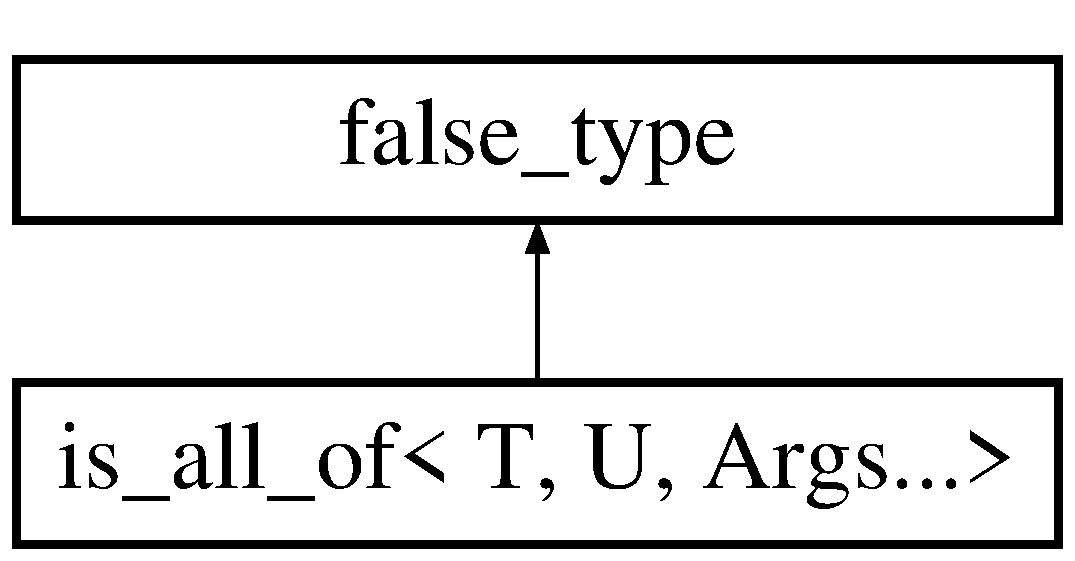
\includegraphics[height=2.000000cm]{structis__all__of_3_01T_00_01U_00_01Args_8_8_8_4}
\end{center}
\end{figure}


\subsection{Detailed Description}
\subsubsection*{template$<$typename T, typename U, typename... Args$>$struct is\-\_\-all\-\_\-of$<$ T, U, Args...$>$}

\hyperlink{structis__all__of}{is\-\_\-all\-\_\-of} meta-\/class. 

Inputs parameter and first parameter are not equal. \begin{DoxyReturn}{Returns}
false 
\end{DoxyReturn}


The documentation for this struct was generated from the following file\-:\begin{DoxyCompactItemize}
\item 
\hyperlink{print__ip_8h}{print\-\_\-ip.\-h}\end{DoxyCompactItemize}

\hypertarget{structis__one__of}{\section{is\-\_\-one\-\_\-of$<$ T, Args $>$ Struct Template Reference}
\label{structis__one__of}\index{is\-\_\-one\-\_\-of$<$ T, Args $>$@{is\-\_\-one\-\_\-of$<$ T, Args $>$}}
}


\hyperlink{structis__one__of}{is\-\_\-one\-\_\-of} meta-\/class.  




{\ttfamily \#include $<$print\-\_\-ip.\-h$>$}



\subsection{Detailed Description}
\subsubsection*{template$<$typename T, typename... Args$>$struct is\-\_\-one\-\_\-of$<$ T, Args $>$}

\hyperlink{structis__one__of}{is\-\_\-one\-\_\-of} meta-\/class. 

A basic class of \hyperlink{structis__one__of}{is\-\_\-one\-\_\-of} meta-\/function. 

The documentation for this struct was generated from the following file\-:\begin{DoxyCompactItemize}
\item 
\hyperlink{print__ip_8h}{print\-\_\-ip.\-h}\end{DoxyCompactItemize}

\hypertarget{structis__one__of_3_01T_01_4}{\section{is\-\_\-one\-\_\-of$<$ T $>$ Struct Template Reference}
\label{structis__one__of_3_01T_01_4}\index{is\-\_\-one\-\_\-of$<$ T $>$@{is\-\_\-one\-\_\-of$<$ T $>$}}
}


\hyperlink{structis__one__of}{is\-\_\-one\-\_\-of} meta-\/class.  




{\ttfamily \#include $<$print\-\_\-ip.\-h$>$}

Inheritance diagram for is\-\_\-one\-\_\-of$<$ T $>$\-:\begin{figure}[H]
\begin{center}
\leavevmode
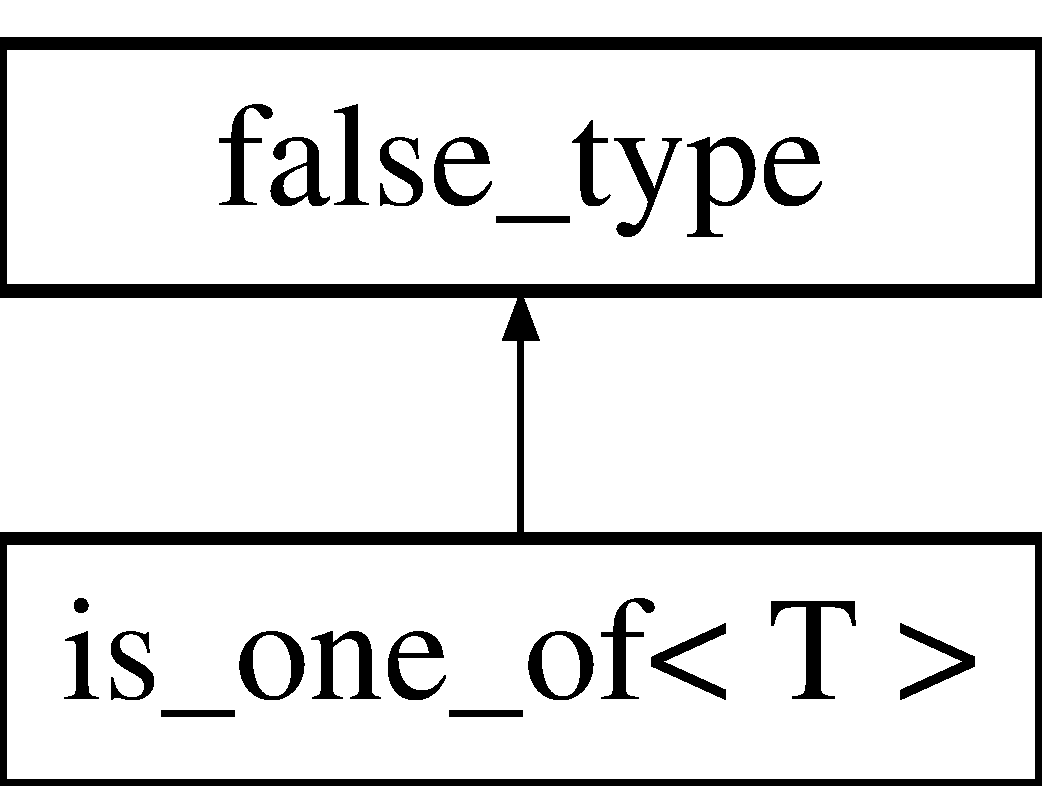
\includegraphics[height=2.000000cm]{structis__one__of_3_01T_01_4}
\end{center}
\end{figure}


\subsection{Detailed Description}
\subsubsection*{template$<$typename T$>$struct is\-\_\-one\-\_\-of$<$ T $>$}

\hyperlink{structis__one__of}{is\-\_\-one\-\_\-of} meta-\/class. 

No parameters. \begin{DoxyReturn}{Returns}
false 
\end{DoxyReturn}


The documentation for this struct was generated from the following file\-:\begin{DoxyCompactItemize}
\item 
\hyperlink{print__ip_8h}{print\-\_\-ip.\-h}\end{DoxyCompactItemize}

\hypertarget{structis__one__of_3_01T_00_01T_00_01Args_8_8_8_4}{\section{is\-\_\-one\-\_\-of$<$ T, T, Args...$>$ Struct Template Reference}
\label{structis__one__of_3_01T_00_01T_00_01Args_8_8_8_4}\index{is\-\_\-one\-\_\-of$<$ T, T, Args...$>$@{is\-\_\-one\-\_\-of$<$ T, T, Args...$>$}}
}


\hyperlink{structis__one__of}{is\-\_\-one\-\_\-of} meta-\/class.  




{\ttfamily \#include $<$print\-\_\-ip.\-h$>$}

Inheritance diagram for is\-\_\-one\-\_\-of$<$ T, T, Args...$>$\-:\begin{figure}[H]
\begin{center}
\leavevmode
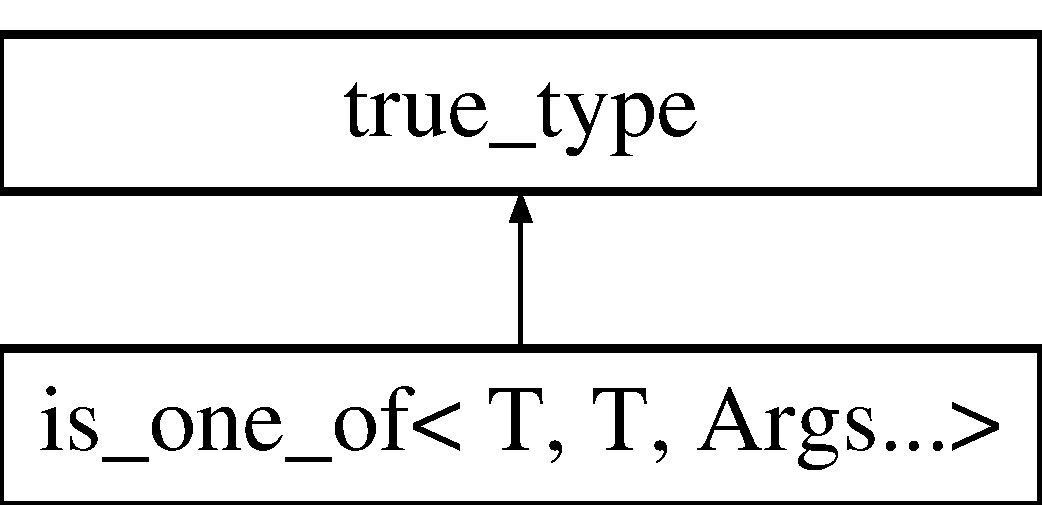
\includegraphics[height=2.000000cm]{structis__one__of_3_01T_00_01T_00_01Args_8_8_8_4}
\end{center}
\end{figure}


\subsection{Detailed Description}
\subsubsection*{template$<$typename T, typename... Args$>$struct is\-\_\-one\-\_\-of$<$ T, T, Args...$>$}

\hyperlink{structis__one__of}{is\-\_\-one\-\_\-of} meta-\/class. 

Inputs parameter and first parameter are equal. \begin{DoxyReturn}{Returns}
true 
\end{DoxyReturn}


The documentation for this struct was generated from the following file\-:\begin{DoxyCompactItemize}
\item 
\hyperlink{print__ip_8h}{print\-\_\-ip.\-h}\end{DoxyCompactItemize}

\hypertarget{structis__one__of_3_01T_00_01U_00_01Args_8_8_8_4}{\section{is\-\_\-one\-\_\-of$<$ T, U, Args...$>$ Struct Template Reference}
\label{structis__one__of_3_01T_00_01U_00_01Args_8_8_8_4}\index{is\-\_\-one\-\_\-of$<$ T, U, Args...$>$@{is\-\_\-one\-\_\-of$<$ T, U, Args...$>$}}
}


\hyperlink{structis__one__of}{is\-\_\-one\-\_\-of} meta-\/class.  




{\ttfamily \#include $<$print\-\_\-ip.\-h$>$}

Inheritance diagram for is\-\_\-one\-\_\-of$<$ T, U, Args...$>$\-:\begin{figure}[H]
\begin{center}
\leavevmode
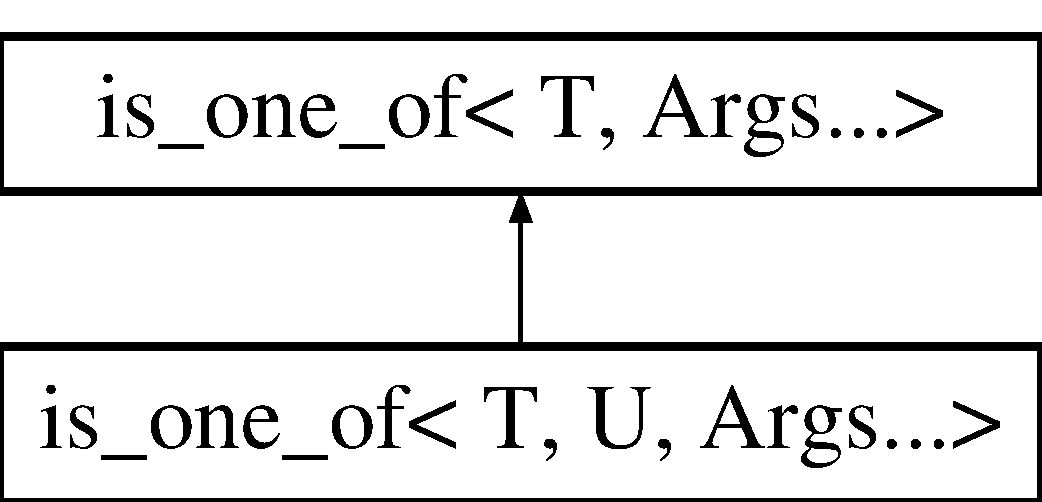
\includegraphics[height=2.000000cm]{structis__one__of_3_01T_00_01U_00_01Args_8_8_8_4}
\end{center}
\end{figure}


\subsection{Detailed Description}
\subsubsection*{template$<$typename T, typename U, typename... Args$>$struct is\-\_\-one\-\_\-of$<$ T, U, Args...$>$}

\hyperlink{structis__one__of}{is\-\_\-one\-\_\-of} meta-\/class. 

Inputs parameter and first parameter are not equal. \begin{DoxyReturn}{Returns}
next compared inputs parameter with second parameter 
\end{DoxyReturn}


The documentation for this struct was generated from the following file\-:\begin{DoxyCompactItemize}
\item 
\hyperlink{print__ip_8h}{print\-\_\-ip.\-h}\end{DoxyCompactItemize}

\hypertarget{structseq}{\section{seq$<$ Is $>$ Struct Template Reference}
\label{structseq}\index{seq$<$ Is $>$@{seq$<$ Is $>$}}
}


seq meta-\/class.  




{\ttfamily \#include $<$print\-\_\-ip.\-h$>$}



\subsection{Detailed Description}
\subsubsection*{template$<$std\-::size\-\_\-t... Is$>$struct seq$<$ Is $>$}

seq meta-\/class. 

Sequence meta-\/function. 

The documentation for this struct was generated from the following file\-:\begin{DoxyCompactItemize}
\item 
\hyperlink{print__ip_8h}{print\-\_\-ip.\-h}\end{DoxyCompactItemize}

\chapter{File Documentation}
\hypertarget{print__ip_8h}{\section{print\-\_\-ip.\-h File Reference}
\label{print__ip_8h}\index{print\-\_\-ip.\-h@{print\-\_\-ip.\-h}}
}
{\ttfamily \#include \char`\"{}version.\-h\char`\"{}}\\*
{\ttfamily \#include $<$cstdint$>$}\\*
{\ttfamily \#include $<$iostream$>$}\\*
{\ttfamily \#include $<$type\-\_\-traits$>$}\\*
{\ttfamily \#include $<$vector$>$}\\*
{\ttfamily \#include $<$list$>$}\\*
{\ttfamily \#include $<$tuple$>$}\\*
{\ttfamily \#include $<$arpa/inet.\-h$>$}\\*
\subsection*{Classes}
\begin{DoxyCompactItemize}
\item 
struct \hyperlink{structis__one__of}{is\-\_\-one\-\_\-of$<$ T, Args $>$}
\begin{DoxyCompactList}\small\item\em \hyperlink{structis__one__of}{is\-\_\-one\-\_\-of} meta-\/class. \end{DoxyCompactList}\item 
struct \hyperlink{structis__one__of_3_01T_01_4}{is\-\_\-one\-\_\-of$<$ T $>$}
\begin{DoxyCompactList}\small\item\em \hyperlink{structis__one__of}{is\-\_\-one\-\_\-of} meta-\/class. \end{DoxyCompactList}\item 
struct \hyperlink{structis__one__of_3_01T_00_01T_00_01Args_8_8_8_4}{is\-\_\-one\-\_\-of$<$ T, T, Args...$>$}
\begin{DoxyCompactList}\small\item\em \hyperlink{structis__one__of}{is\-\_\-one\-\_\-of} meta-\/class. \end{DoxyCompactList}\item 
struct \hyperlink{structis__one__of_3_01T_00_01U_00_01Args_8_8_8_4}{is\-\_\-one\-\_\-of$<$ T, U, Args...$>$}
\begin{DoxyCompactList}\small\item\em \hyperlink{structis__one__of}{is\-\_\-one\-\_\-of} meta-\/class. \end{DoxyCompactList}\item 
struct \hyperlink{structseq}{seq$<$ Is $>$}
\begin{DoxyCompactList}\small\item\em seq meta-\/class. \end{DoxyCompactList}\item 
struct \hyperlink{structgen__seq}{gen\-\_\-seq$<$ N, Is $>$}
\begin{DoxyCompactList}\small\item\em \hyperlink{structgen__seq}{gen\-\_\-seq} meta-\/class. \end{DoxyCompactList}\item 
struct \hyperlink{structgen__seq_3_010_00_01Is_8_8_8_4}{gen\-\_\-seq$<$ 0, Is...$>$}
\begin{DoxyCompactList}\small\item\em \hyperlink{structgen__seq}{gen\-\_\-seq} meta-\/class. \end{DoxyCompactList}\item 
struct \hyperlink{structis__all__of}{is\-\_\-all\-\_\-of$<$ T, Args $>$}
\begin{DoxyCompactList}\small\item\em \hyperlink{structis__all__of}{is\-\_\-all\-\_\-of} meta-\/class. \end{DoxyCompactList}\item 
struct \hyperlink{structis__all__of_3_01T_01_4}{is\-\_\-all\-\_\-of$<$ T $>$}
\begin{DoxyCompactList}\small\item\em \hyperlink{structis__all__of}{is\-\_\-all\-\_\-of} meta-\/class. \end{DoxyCompactList}\item 
struct \hyperlink{structis__all__of_3_01T_00_01U_00_01Args_8_8_8_4}{is\-\_\-all\-\_\-of$<$ T, U, Args...$>$}
\begin{DoxyCompactList}\small\item\em \hyperlink{structis__all__of}{is\-\_\-all\-\_\-of} meta-\/class. \end{DoxyCompactList}\item 
struct \hyperlink{structis__all__of_3_01T_00_01T_00_01Args_8_8_8_4}{is\-\_\-all\-\_\-of$<$ T, T, Args...$>$}
\begin{DoxyCompactList}\small\item\em \hyperlink{structis__all__of}{is\-\_\-all\-\_\-of} meta-\/class. \end{DoxyCompactList}\end{DoxyCompactItemize}
\subsection*{Functions}
\begin{DoxyCompactItemize}
\item 
int \hyperlink{print__ip_8h_ae64f17a84dc9c7144d1036498ff26fd9}{version} ()
\begin{DoxyCompactList}\small\item\em version function. \end{DoxyCompactList}\item 
{\footnotesize template$<$typename T $>$ }\\std\-::enable\-\_\-if\-\_\-t$<$ \hyperlink{print__ip_8h_a43d3c463d00de7c3fc5d6e1655f691cd}{is\-\_\-one\-\_\-of\-\_\-v}\\*
$<$ T, std\-::int8\-\_\-t, std\-::uint8\-\_\-t, \\*
std\-::int16\-\_\-t, std\-::uint16\-\_\-t, \\*
std\-::int32\-\_\-t, std\-::uint32\-\_\-t, \\*
std\-::int64\-\_\-t, std\-::uint64\-\_\-t $>$\\*
, void $>$ \hyperlink{print__ip_8h_aaf19367a3ba874c55a1071c86cfa774e}{print\-\_\-ip} (const T \&ip)
\begin{DoxyCompactList}\small\item\em Template print\-\_\-ip taking one argument which is one of integer type and print it as ip-\/address (bytes sepated by dots). \end{DoxyCompactList}\item 
{\footnotesize template$<$template$<$ typename, typename $>$ class T, typename U $>$ }\\std\-::enable\-\_\-if\-\_\-t$<$ \hyperlink{print__ip_8h_a43d3c463d00de7c3fc5d6e1655f691cd}{is\-\_\-one\-\_\-of\-\_\-v}\\*
$<$ T$<$ U, std\-::allocator$<$ U $>$\\*
 $>$, std\-::vector$<$ U $>$\\*
, std\-::list$<$ U $>$ $>$, void $>$ \hyperlink{print__ip_8h_a8da9671c7dca68b86537a8de5cf0898c}{print\-\_\-ip} (const T$<$ U, std\-::allocator$<$ U $>$$>$ \&ip)
\begin{DoxyCompactList}\small\item\em Template print\-\_\-ip taking one argument which is one of std\-::vector or std\-::list type and print it as ip-\/address (bytes sepated by dots). \end{DoxyCompactList}\item 
{\footnotesize template$<$typename Ch , typename Tr , typename Tuple , std\-::size\-\_\-t... Is$>$ }\\void \hyperlink{print__ip_8h_aab22855dd4e319ef4b17b7c303f097ec}{print\-\_\-tuple} (std\-::basic\-\_\-ostream$<$ Ch, Tr $>$ \&os, Tuple const \&t, \hyperlink{structseq}{seq}$<$ Is...$>$)
\begin{DoxyCompactList}\small\item\em Template print\-\_\-tuple taking three arguments (one of these parameters is a tuple) and print it as ip-\/address (bytes sepated by dots). \end{DoxyCompactList}\item 
{\footnotesize template$<$typename Ch , typename Tr , typename... Args$>$ }\\auto \hyperlink{print__ip_8h_a2c4f4bc09a3bd265112bc2774b86341c}{operator$<$$<$} (std\-::basic\-\_\-ostream$<$ Ch, Tr $>$ \&os, std\-::tuple$<$ Args...$>$ const \&t) -\/$>$ std\-::basic\-\_\-ostream$<$ Ch, Tr $>$ \&
\begin{DoxyCompactList}\small\item\em Overloaded operator \char`\"{}$<$$<$\char`\"{} template taking two arguments (one of these parameters is a tuple) and put it to std output. \end{DoxyCompactList}\item 
{\footnotesize template$<$typename... Args$>$ }\\std\-::enable\-\_\-if\-\_\-t$<$ \hyperlink{print__ip_8h_a4e2e58f599cd0aded1b1c451e2bf4ddf}{is\-\_\-all\-\_\-of\-\_\-v}\\*
$<$ Args...$>$, void $>$ \hyperlink{print__ip_8h_a49c1450a299777cd37de84f266f5417b}{print\-\_\-ip} (std\-::tuple$<$ Args...$>$ const \&ip)
\begin{DoxyCompactList}\small\item\em Template print\-\_\-ip taking one tuple-\/parameter. \end{DoxyCompactList}\end{DoxyCompactItemize}
\subsection*{Variables}
\begin{DoxyCompactItemize}
\item 
\hypertarget{print__ip_8h_a43d3c463d00de7c3fc5d6e1655f691cd}{{\footnotesize template$<$typename T , typename U , typename... Args$>$ }\\constexpr bool \hyperlink{print__ip_8h_a43d3c463d00de7c3fc5d6e1655f691cd}{is\-\_\-one\-\_\-of\-\_\-v} = \hyperlink{structis__one__of}{is\-\_\-one\-\_\-of}$<$T, U, Args...$>$\-::value}\label{print__ip_8h_a43d3c463d00de7c3fc5d6e1655f691cd}

\begin{DoxyCompactList}\small\item\em \hyperlink{structis__one__of}{is\-\_\-one\-\_\-of} meta-\/class value alias. \end{DoxyCompactList}\item 
\hypertarget{print__ip_8h_a4e2e58f599cd0aded1b1c451e2bf4ddf}{{\footnotesize template$<$typename T , typename... Args$>$ }\\constexpr bool \hyperlink{print__ip_8h_a4e2e58f599cd0aded1b1c451e2bf4ddf}{is\-\_\-all\-\_\-of\-\_\-v} = \hyperlink{structis__all__of}{is\-\_\-all\-\_\-of}$<$T, Args...$>$\-::value}\label{print__ip_8h_a4e2e58f599cd0aded1b1c451e2bf4ddf}

\begin{DoxyCompactList}\small\item\em \hyperlink{structis__all__of}{is\-\_\-all\-\_\-of} meta-\/class value alias. \end{DoxyCompactList}\end{DoxyCompactItemize}


\subsection{Function Documentation}
\hypertarget{print__ip_8h_a2c4f4bc09a3bd265112bc2774b86341c}{\index{print\-\_\-ip.\-h@{print\-\_\-ip.\-h}!operator$<$$<$@{operator$<$$<$}}
\index{operator$<$$<$@{operator$<$$<$}!print_ip.h@{print\-\_\-ip.\-h}}
\subsubsection[{operator$<$$<$}]{\setlength{\rightskip}{0pt plus 5cm}template$<$typename Ch , typename Tr , typename... Args$>$ auto operator$<$$<$ (
\begin{DoxyParamCaption}
\item[{std\-::basic\-\_\-ostream$<$ Ch, Tr $>$ \&}]{os, }
\item[{std\-::tuple$<$ Args...$>$ const \&}]{t}
\end{DoxyParamCaption}
) -\/$>$ std\-::basic\-\_\-ostream$<$Ch, Tr$>$\&
}}\label{print__ip_8h_a2c4f4bc09a3bd265112bc2774b86341c}


Overloaded operator \char`\"{}$<$$<$\char`\"{} template taking two arguments (one of these parameters is a tuple) and put it to std output. 


\begin{DoxyParams}[1]{Parameters}
\mbox{\tt out}  & {\em os} & an std\-::basic\-\_\-ostream$<$$>$ argument, such as std\-::cout. \\
\hline
\mbox{\tt in}  & {\em t} & a std\-::tuple argument, it's ip address. \\
\hline
\end{DoxyParams}
\begin{DoxyReturn}{Returns}
std\-::basic\-\_\-ostream$<$$>$ variable 
\end{DoxyReturn}
\hypertarget{print__ip_8h_aaf19367a3ba874c55a1071c86cfa774e}{\index{print\-\_\-ip.\-h@{print\-\_\-ip.\-h}!print\-\_\-ip@{print\-\_\-ip}}
\index{print\-\_\-ip@{print\-\_\-ip}!print_ip.h@{print\-\_\-ip.\-h}}
\subsubsection[{print\-\_\-ip}]{\setlength{\rightskip}{0pt plus 5cm}template$<$typename T $>$ std\-::enable\-\_\-if\-\_\-t$<${\bf is\-\_\-one\-\_\-of\-\_\-v}$<$T, std\-::int8\-\_\-t, std\-::uint8\-\_\-t, std\-::int16\-\_\-t, std\-::uint16\-\_\-t, std\-::int32\-\_\-t, std\-::uint32\-\_\-t, std\-::int64\-\_\-t, std\-::uint64\-\_\-t$>$, void$>$ print\-\_\-ip (
\begin{DoxyParamCaption}
\item[{const T \&}]{ip}
\end{DoxyParamCaption}
)}}\label{print__ip_8h_aaf19367a3ba874c55a1071c86cfa774e}


Template print\-\_\-ip taking one argument which is one of integer type and print it as ip-\/address (bytes sepated by dots). 


\begin{DoxyParams}[1]{Parameters}
\mbox{\tt in}  & {\em ip} & an integer argument. \\
\hline
\end{DoxyParams}
\hypertarget{print__ip_8h_a8da9671c7dca68b86537a8de5cf0898c}{\index{print\-\_\-ip.\-h@{print\-\_\-ip.\-h}!print\-\_\-ip@{print\-\_\-ip}}
\index{print\-\_\-ip@{print\-\_\-ip}!print_ip.h@{print\-\_\-ip.\-h}}
\subsubsection[{print\-\_\-ip}]{\setlength{\rightskip}{0pt plus 5cm}template$<$template$<$ typename, typename $>$ class T, typename U $>$ std\-::enable\-\_\-if\-\_\-t$<${\bf is\-\_\-one\-\_\-of\-\_\-v}$<$T$<$U, std\-::allocator$<$U$>$ $>$, std\-::vector$<$U$>$, std\-::list$<$U$>$ $>$, void$>$ print\-\_\-ip (
\begin{DoxyParamCaption}
\item[{const T$<$ U, std\-::allocator$<$ U $>$$>$ \&}]{ip}
\end{DoxyParamCaption}
)}}\label{print__ip_8h_a8da9671c7dca68b86537a8de5cf0898c}


Template print\-\_\-ip taking one argument which is one of std\-::vector or std\-::list type and print it as ip-\/address (bytes sepated by dots). 


\begin{DoxyParams}[1]{Parameters}
\mbox{\tt in}  & {\em ip} & an std\-::vector or std\-::list argument. \\
\hline
\end{DoxyParams}
\hypertarget{print__ip_8h_a49c1450a299777cd37de84f266f5417b}{\index{print\-\_\-ip.\-h@{print\-\_\-ip.\-h}!print\-\_\-ip@{print\-\_\-ip}}
\index{print\-\_\-ip@{print\-\_\-ip}!print_ip.h@{print\-\_\-ip.\-h}}
\subsubsection[{print\-\_\-ip}]{\setlength{\rightskip}{0pt plus 5cm}template$<$typename... Args$>$ std\-::enable\-\_\-if\-\_\-t$<${\bf is\-\_\-all\-\_\-of\-\_\-v}$<$Args...$>$, void$>$ print\-\_\-ip (
\begin{DoxyParamCaption}
\item[{std\-::tuple$<$ Args...$>$ const \&}]{ip}
\end{DoxyParamCaption}
)}}\label{print__ip_8h_a49c1450a299777cd37de84f266f5417b}


Template print\-\_\-ip taking one tuple-\/parameter. 


\begin{DoxyParams}[1]{Parameters}
\mbox{\tt in}  & {\em ip} & a std\-::tuple argument, it's ip address. \\
\hline
\end{DoxyParams}
\hypertarget{print__ip_8h_aab22855dd4e319ef4b17b7c303f097ec}{\index{print\-\_\-ip.\-h@{print\-\_\-ip.\-h}!print\-\_\-tuple@{print\-\_\-tuple}}
\index{print\-\_\-tuple@{print\-\_\-tuple}!print_ip.h@{print\-\_\-ip.\-h}}
\subsubsection[{print\-\_\-tuple}]{\setlength{\rightskip}{0pt plus 5cm}template$<$typename Ch , typename Tr , typename Tuple , std\-::size\-\_\-t... Is$>$ void print\-\_\-tuple (
\begin{DoxyParamCaption}
\item[{std\-::basic\-\_\-ostream$<$ Ch, Tr $>$ \&}]{os, }
\item[{Tuple const \&}]{t, }
\item[{{\bf seq}$<$ Is...$>$}]{}
\end{DoxyParamCaption}
)}}\label{print__ip_8h_aab22855dd4e319ef4b17b7c303f097ec}


Template print\-\_\-tuple taking three arguments (one of these parameters is a tuple) and print it as ip-\/address (bytes sepated by dots). 


\begin{DoxyParams}[1]{Parameters}
\mbox{\tt out}  & {\em os} & an std\-::basic\-\_\-ostream$<$$>$ argument, such as std\-::cout. \\
\hline
\mbox{\tt in}  & {\em t} & a std\-::tuple argument, it's ip address. \\
\hline
\mbox{\tt in}  & {\em seq$<$\-Is...$>$} & a metaprogramming-\/generated sequence of integer numbers (0..N) argument, it's according to tuple indexes. \\
\hline
\end{DoxyParams}
\hypertarget{print__ip_8h_ae64f17a84dc9c7144d1036498ff26fd9}{\index{print\-\_\-ip.\-h@{print\-\_\-ip.\-h}!version@{version}}
\index{version@{version}!print_ip.h@{print\-\_\-ip.\-h}}
\subsubsection[{version}]{\setlength{\rightskip}{0pt plus 5cm}int version (
\begin{DoxyParamCaption}
{}
\end{DoxyParamCaption}
)}}\label{print__ip_8h_ae64f17a84dc9c7144d1036498ff26fd9}


version function. 

\begin{DoxyReturn}{Returns}
int value $>$ 0 
\end{DoxyReturn}

%--- End generated contents ---

% Index
\newpage
\phantomsection
\addcontentsline{toc}{chapter}{Index}
\printindex

\end{document}
